%-----------------------------------------------------------------------------%
\chapter{\babTiga}
%-----------------------------------------------------------------------------%

Dari permasalahan yang sudah didefinisikan, maka akan dibuat sebuah program yang akan melakukan integrasi ontologi dan \textit{web service} dengan memanfaatkan Zotonic. Sebelum memulai pembuatan program, perlu dirancang bagaimana program ini akan berjalan. Pada bab ini, akan dibahas mengenai rancangan integrasi ontologi dan \textit{web service} yang akan menggambarkan secara keseluruhan bagaimana program akan bekerja serta hal lainnya yang terhubungan dengan program dan juga mengenai rancangan adaptor yang akan menggambarkan secara dalam bagaimana program dapat mengakses \textit{web service} dan terhubung dengan ontologi.
%-----------------------------------------------------------------------------%
\section{Rancangan Integrasi Ontologi dan \textit{Web Service}}
%-----------------------------------------------------------------------------%

Agar dapat menghasilkan program yang bertujuan untuk melakukan integrasi ontologi dan \textit{web services} maka perlu dirancang secara keseluruhan bagaimana program ini akan bekerja. Sesuai dengan kebutuhan dari program, maka integrasi ini akan dilakukan pada sebuah \textit{framework} sekaligus \textit{CMS} Zotonic, yang telah dimodifikasi agar dapat menerima masukan berupa ontologi. Secara garis besar, berikut merupakan gambaran cara program akan bekerja.

\begin{figure}
	\centering
	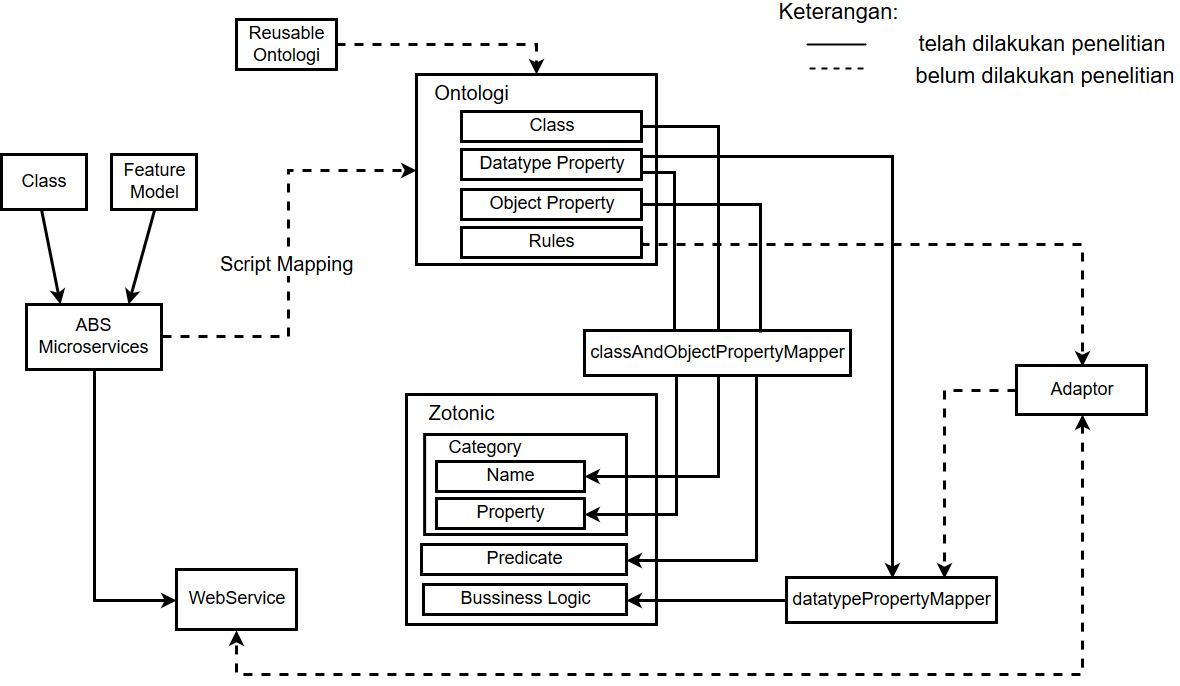
\includegraphics[width=1\textwidth]
		{pics/skripsiRoadmapNew.jpg}
	\caption{Rancangan integrasi ontologi dan web service}
	\label{fig:skripsiroadmap}
\end{figure}
\vspace{-0.3cm}

Seperti yang dapat dilihat pada \pic~\ref{fig:skripsiroadmap}, \textit{Class} dan \textit{Feature Model} akan diproses menggunakan program translasi yang akan menghasilkan ABS \textit{Microservices} dimana ini telah dilakukan penelitian sebelumnya sehingga hal ini bukan merupakan bagian dari penelitian penulis. Setelah dihasilkan sebuah ABS \textit{Microservices} dari proses translasi tersebut, maka ABS \textit{Microservices} akan menghasilkan sebuah \textit{web service} yang dapat digunakan oleh program lainnya. Dalam penelitian ini, \textit{web services} yang dihasilkan oleh ABS \textit{Microservices} akan digunakan oleh \textit{Adaptor} yang akan terhubung dengan Zotonic. Selain digunakan untuk menghasilkan sebuah \textit{web service}, ABS \textit{Microservices} akan digunakan untuk menghasilkan sebuah ontologi menggunakan sebuah \textit{script} yang akan melakukan pemetaan dari \textit{class} dan \textit{feature model} menjadi \textit{class, datatype property, object property} dan \textit{rules} pada ontologi. Untuk pemetaan ini sendiri tidak termasuk dalam penelitian ini karena penulis hanya akan menggunakan sebuah ontologi yang telah dirancang sebelumnya. Nantinya melalui proses pemetaan ini, akan dihasilkan sebuah ontologi yang bersifat \textit{reusable}.

Menggunakan ontologi yang telah dirancang sebelumnya, ontologi tersebut akan dipetakan ke dalam struktur dari zotonic yang akan digunakan. Proses pemetaan dari ontologi ke dalam zotonic ini sendiri telah dilakukan pada penelitian sebelumnya oleh Bravyto dimana setiap \textit{class} dari ontologi akan dipetakan menjadi nama dari kategori pada zotonic menggunakan \textit{script classAndObjectPropertyMapper.sh}. Selain melakukan pemetaan pada \textit{class, script} tersebut juga akan melakukan pemetaan \textit{datatype property} pada ontologi menjadi \textit{property} dari kategori pada zotonic serta pemetaan \textit{object property} pada ontologi menjadi \textit{predicate} pada zotonic. Pada penelitian tersebut, dilakukan juga pemetaan dari \textit{datatype property} menjadi \textit{business logic} menggunakan \textit{script} datatypePropertyMapper.sh.

Namun pada penelitian tersebut, pembuatan \textit{business logic} masih bersifat manual yang langsung ditaruh pada \textit{script} datatypepropertyMapper.sh. Pada penelitian ini, penulis akan membuat sebuah adaptor yang akan memanggil \textit{web service} sehingga \textit{business logic} pada zotonic akan lebih fleksibel karena memanfaatkan \textit{web service} serta memberikan kemudahan bagi \textit{developer} dalam hal melakukan modifikasi.
%-----------------------------------------------------------------------------%
\section{Rancangan \textit{Web Service}}
%-----------------------------------------------------------------------------%

	\todo{Jelasin gimana rancangan API nya.}

%-----------------------------------------------------------------------------%
\section{Rancangan \f{Adaptor}}
%-----------------------------------------------------------------------------%

Adaptor merupakan sebuah \textit{script} yang akan memanggil \textit{web service} sehingga dapat digunakan untuk melakukan pemrosesan \textit{business logic} pada zotonic. Bagaimana adaptor akan bekerja sehingga menghasilkan business logic dapat dilihat pada gambar berikut ini.

\begin{figure}
	\centering
	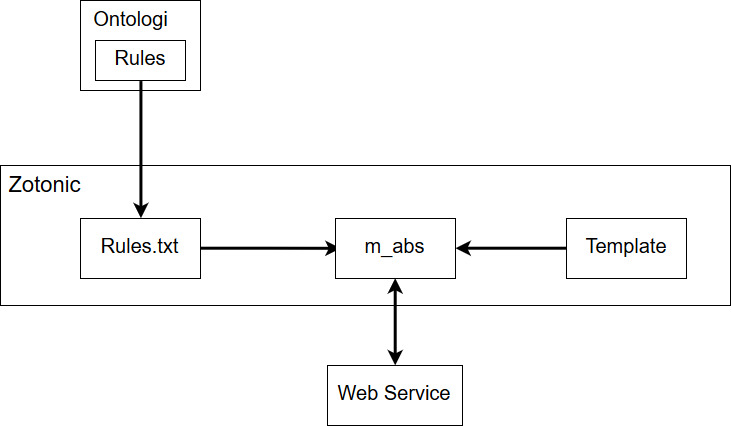
\includegraphics[width=0.7\textwidth]
		{pics/adaptor.jpg}
	\caption{Rancangan Adaptor}
	\label{fig:adaptor}
\end{figure}
\vspace{-0.3cm}

Seperti yang dapat dilihat pada \pic~\ref{fig:adaptor}, \textit{rules} yang terdapat pada ontologi akan dilakukan pemetaan menjadi tabel \textit{rules} yang akan disimpan pada file rules.txt seperti yang terdapat pada kode \ref{lst:tablerules}. Namun, proses pemetaan ini berada diluar dari topik penelitian penulis sehingga untuk keperluan penelitian ini maka penulis membuat sebuah tabel \textit{rules} secara manual untuk mengganti proses pemetaan tersebut.

\begin{minipage}{\linewidth}
\begin{lstlisting}[caption={Contoh tabel \textit{rules}},label={lst:tablerules}]
{
	"createProgram": ["http://54.169.128.6:8080/abs/program/create", 2],
	"createDonation": ["http://54.169.128.6:8080/abs/donation/create", 4],
	"updateProgram": ["http://54.169.128.6:8080/abs/program/update", 2],
	"updateDonation": ["http://54.169.128.6:8080/abs/donation/update", 4],
	"deleteProgram": ["http://54.169.128.6:8080/abs/program/delete", 1],
	"deleteDonation": ["http://54.169.128.6:8080/abs/donation/delete", 1],
	"totalDonation" : ["http://54.169.128.6:8080/abs/program/total-donation", 1]
}
\end{lstlisting}
\end{minipage} \\

Setelah terbentuk tabel \textit{rules} pada file rules.txt, maka ketika model abs yang terdapat pada file dijalankan pada \textit{template engine}, model abs akan membaca \textit{rules} untuk mengetahui \textit{endpoint} yang akan dijalankan pada proses pemanggilan \textit{web service} serta untuk melakukan pengecekan apakah jumlah parameter yang dimasukkan telah sesuai dengan jumlah parameter yang diterima oleh \textit{web service} atau tidak.